%% Generated from exact unmasked Step-ODE and outcome exit trajectories.
\definecolor{stepc}{HTML}{0072B2}\definecolor{outc}{HTML}{D55E00}\definecolor{theoc}{HTML}{009E73}\definecolor{midc}{HTML}{CC79A7}\definecolor{mutedc}{HTML}{6E6E6E}
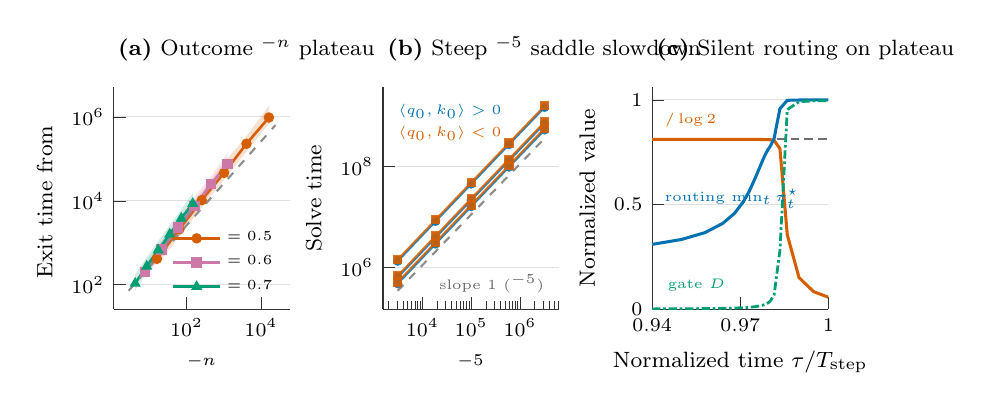
\begin{tikzpicture}
\pgfplotsset{every axis/.style={width=0.315\linewidth, height=4.4cm, axis line style={black!80}, tick style={black!80},
  tick label style={font=\scriptsize}, label style={font=\footnotesize}, title style={font=\footnotesize, at={(0,1)}, anchor=south west, xshift=-2pt},
  axis x line*=bottom, axis y line*=left, ymajorgrids, major grid style={black!12}}, every axis plot/.append style={line width=0.95pt}}
\begin{loglogaxis}[name=pa, title={\textbf{(a)} Outcome $\mixrate^{-n}$ plateau}, xlabel={$\mixrate^{-n}$}, ylabel={Exit time from $\initball$},
  legend style={font=\tiny, draw=none, fill=none, at={(0.98,0.02)}, anchor=south east}, legend cell align=left]
  \addplot[draw=none, fill=outc, fill opacity=0.18, forget plot] coordinates {(16,283.012) (64,1413.23) (256,6857.96) (1024,32201.5) (4096,147996) (16384,689161) (16384,1.83425e+06) (4096,347476) (1024,81811.4) (256,16373.4) (64,3385.08) (16,676.199)};
  \addplot[outc, mark=*, mark size=1.4pt] coordinates {(16,413.863) (64,2084) (256,10375.8) (1024,46257.4) (4096,228645) (16384,964510)};
  \addlegendentry{$\mixrate=0.5$}
  \addplot[draw=none, fill=midc, fill opacity=0.18, forget plot] coordinates {(7.71605,136.439) (21.4335,473.075) (59.5374,1580.02) (165.382,5126.31) (459.394,16396.2) (1276.09,53424.4) (1276.09,142473) (459.394,38943.2) (165.382,12616.4) (59.5374,3785.17) (21.4335,1132.53) (7.71605,325.944)};
  \addplot[midc, mark=square*, mark size=1.4pt] coordinates {(7.71605,198.99) (21.4335,691.557) (59.5374,2333.01) (165.382,7444.27) (459.394,25414.7) (1276.09,75030.9)};
  \addlegendentry{$\mixrate=0.6$}
  \addplot[draw=none, fill=theoc, fill opacity=0.18, forget plot] coordinates {(4.16493,73.6358) (8.49986,187.581) (17.3467,459.286) (35.4013,1092.83) (72.2476,2551.12) (147.444,5945.42) (147.444,15264.5) (72.2476,6115.4) (35.4013,2639.29) (17.3467,1100.71) (8.49986,448.967) (4.16493,175.9)};
  \addplot[theoc, mark=triangle*, mark size=1.4pt] coordinates {(4.16493,107.269) (8.49986,273.487) (17.3467,671.624) (35.4013,1590.59) (72.2476,3811.26) (147.444,8579.4)};
  \addlegendentry{$\mixrate=0.7$}
  \addplot[black!45, dashed, line width=0.75pt, forget plot] coordinates {(2.77662,71.8213) (24576,635694)};
\end{loglogaxis}
\begin{loglogaxis}[name=pb, at={(pa.east)}, anchor=west, xshift=1.18cm, title={\textbf{(b)} Steep $\initscale^{-5}$ saddle slowdown},
  xlabel={$\initscale^{-5}$}, ylabel={Solve time}]
  \addplot[stepc, mark=*, mark size=1.3pt, line width=0.7pt, opacity=0.85] coordinates {(3125,1.340e+06) (18593.4,8.169e+06) (100000,4.468e+07) (594990.2,2.692e+08) (3.2e+06,1.461e+09)};
  \addplot[stepc, mark=*, mark size=1.3pt, line width=0.7pt, opacity=0.85] coordinates {(3125,6.419e+05) (18593.4,3.916e+06) (100000,2.142e+07) (594990.2,1.291e+08) (3.2e+06,7.007e+08)};
  \addplot[stepc, mark=*, mark size=1.3pt, line width=0.7pt, opacity=0.85] coordinates {(3125,4.802e+05) (18593.4,2.931e+06) (100000,1.605e+07) (594990.2,9.676e+07) (3.2e+06,5.252e+08)};
  \addplot[outc, mark=square*, mark size=1.3pt, line width=0.7pt, opacity=0.85] coordinates {(3125,1.451e+06) (18593.4,8.831e+06) (100000,4.824e+07) (594990.2,2.904e+08) (3.2e+06,1.574e+09)};
  \addplot[outc, mark=square*, mark size=1.3pt, line width=0.7pt, opacity=0.85] coordinates {(3125,6.953e+05) (18593.4,4.233e+06) (100000,2.313e+07) (594990.2,1.393e+08) (3.2e+06,7.553e+08)};
  \addplot[outc, mark=square*, mark size=1.3pt, line width=0.7pt, opacity=0.85] coordinates {(3125,5.202e+05) (18593.4,3.170e+06) (100000,1.733e+07) (594990.2,1.044e+08) (3.2e+06,5.662e+08)};
  \addplot[black!45, dashed, line width=0.75pt] coordinates {(3125,3.5e+05) (3.2e+06,3.584e+08)};
  \node[anchor=north west, font=\tiny, text=stepc] at (rel axis cs:0.03,0.97) {$\langle q_0,k_0\rangle > 0$};
  \node[anchor=north west, font=\tiny, text=outc] at (rel axis cs:0.03,0.87) {$\langle q_0,k_0\rangle < 0$};
  \node[anchor=south east, font=\tiny, text=black!60] at (rel axis cs:0.97,0.03) {slope $1$ ($\initscale^{-5}$)};
\end{loglogaxis}
\begin{axis}[name=pc, at={(pb.east)}, anchor=west, xshift=1.18cm, title={\textbf{(c)} Silent routing on plateau},
  xlabel={Normalized time $\tau / T_{\mathrm{step}}$}, ylabel={Normalized value},
  xmin=0.94, xmax=1.00, ymin=0, ymax=1.06, xtick={0.94,0.97,1.00}, ytick={0,0.5,1.0}]
  \addplot[mutedc, densely dashed, line width=0.7pt, domain=0.94:1.00, samples=2] {0.8113};
  \addplot[outc, line width=1.1pt] coordinates {(0.94,0.8113) (0.95,0.8113) (0.958,0.8113) (0.964,0.8112) (0.968,0.8112) (0.971,0.8112) (0.973,0.8111) (0.975,0.811) (0.9765,0.8109) (0.9775,0.8107) (0.9782,0.8105) (0.9788,0.8103) (0.9794,0.81) (0.9802,0.8094) (0.9815,0.8068) (0.9835,0.7675) (0.986,0.3561) (0.99,0.151) (0.995,0.0838) (1.0,0.0575)};
  \addplot[stepc, line width=1.1pt] coordinates {(0.94,0.3099) (0.95,0.3333) (0.958,0.3662) (0.964,0.4099) (0.968,0.4576) (0.971,0.5124) (0.973,0.5622) (0.975,0.624) (0.9765,0.6736) (0.9775,0.7072) (0.9782,0.7296) (0.9788,0.7466) (0.9794,0.7614) (0.9802,0.7786) (0.9815,0.8151) (0.9835,0.9575) (0.986,0.998) (0.99,0.9994) (0.995,0.9997) (1.0,0.9997)};
  \addplot[theoc, densely dashdotted, line width=1.0pt] coordinates {(0.94,0.0017) (0.95,0.0023) (0.958,0.0032) (0.964,0.0044) (0.968,0.0058) (0.971,0.0076) (0.973,0.0094) (0.975,0.0123) (0.9765,0.0156) (0.9775,0.0188) (0.9782,0.022) (0.9788,0.0256) (0.9794,0.0301) (0.9802,0.0385) (0.9815,0.0667) (0.9835,0.2808) (0.986,0.9537) (0.99,0.991) (0.995,0.9954) (1.0,0.9967)};
  \node[anchor=south west, font=\tiny, text=outc] at (axis cs:0.941,0.825) {$\Lstep/\log 2$};
  \node[anchor=north west, font=\tiny, text=stepc] at (axis cs:0.941,0.62) {routing $\min_t\pi_t^\star$};
  \node[anchor=south west, font=\tiny, text=theoc] at (axis cs:0.942,0.04) {gate $D$};
\end{axis}
\end{tikzpicture}
